%\addchap{Appendix}
\chapter{Appendix}
\label{appendix0}

Introductory words that explain the stuff covered here.
Lorem ipsum.

\newpage
\vspace*{1ex}
\section{Moore's law}
\label{appendix1}

\begin{quote} \textit{``The complexity for minimum component costs has increased at a rate of roughly a factor of two per year.''} \citep[p.115]{Moore1965} \end{quote}
Moore’s law is really an economic law stating that the density of transistors must double every 18 to 24 months to enable an economic return from the investment in semiconductor foundries (see figure \ref{fig:moores_law} below for historical data).
Thus it would be wrong to state that the performance of a chip doubles at this rate.
%Bild
\begin{figure}[ht]
\centering
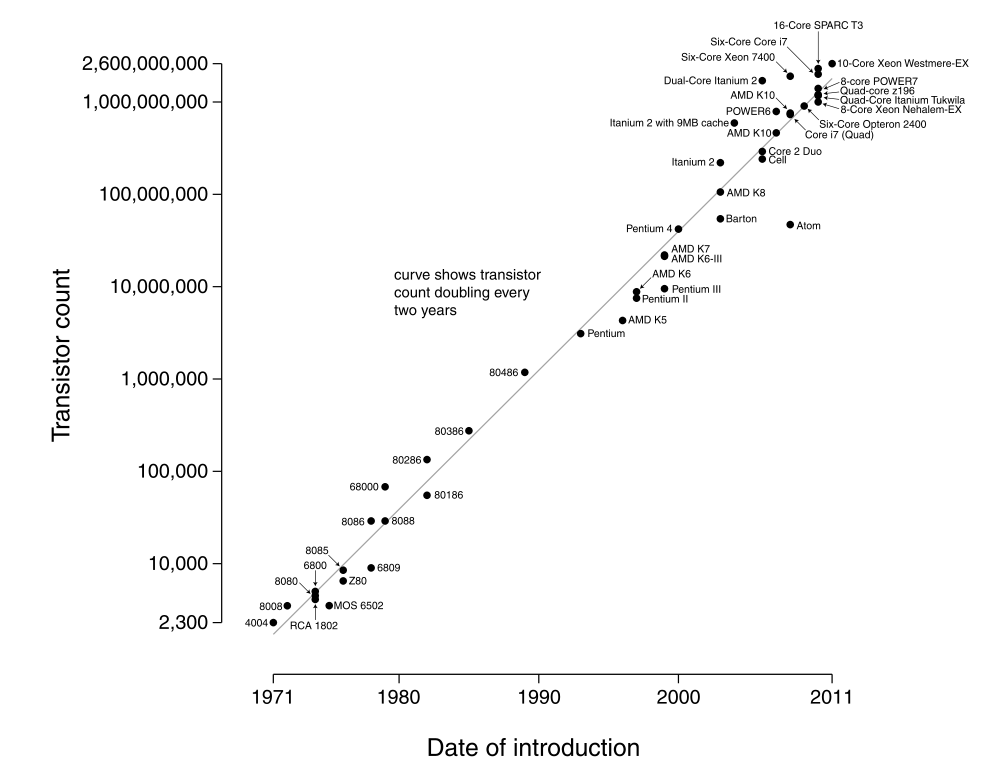
\includegraphics[width=0.66\textwidth]{moores_law.png}
\caption{Microprocessor transistor counts 1971-2011 \& Moore's Law}
\label{fig:moores_law}
\end{figure}\\
The more widely it became accepted, the more it served as a goal for an entire industry.
This drove both marketing and engineering departments of semiconductor manufacturers to focus enormous energy aiming for the specified increase in processing power that it was presumed one or more of their competitors would soon actually attain.
In this regard, it can be viewed as a self-fulfilling prophecy \citep[cf.][]{Paul2006, Crvelin2012}.


\newpage
%\vspace*{1ex}
\section{RenderMen timeline}
\label{appendix2}

During his keynote speech, to kick off Siggraph 2008, Ed Catmull presented the audience with the following timeline detailing the critical advances in rendering technology over the last 20 years at Pixar \citep[cf.][]{Seymour2008}.
\begin{figure}[ht]
\centering
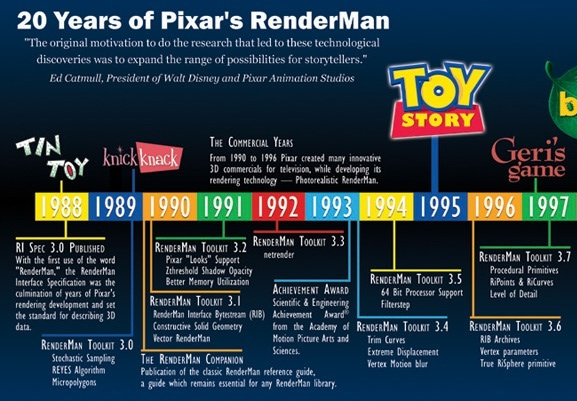
\includegraphics[width=0.78\textwidth]{renderman_timeline_1.jpg}
\caption{20 Years of Pixar's RenderMan - 1}
\label{fig:renderman_timeline_1}
\end{figure}
\begin{figure}[ht]
\centering
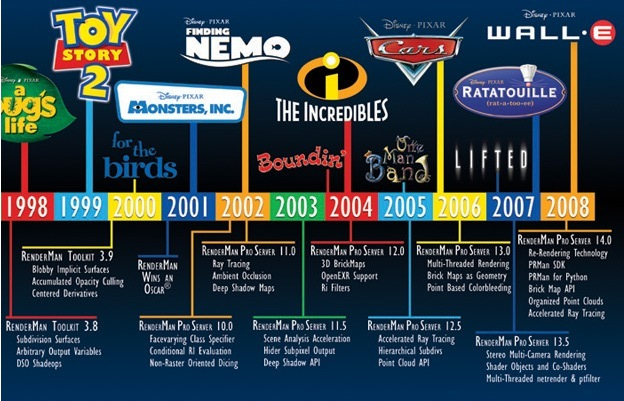
\includegraphics[width=0.78\textwidth]{renderman_timeline_2.jpg}
\caption{20 Years of Pixar's RenderMan - 2}
\label{fig:renderman_timeline_2}
\end{figure}


\newpage
\vspace*{1ex}
\section{The Utah Teapot}
\label{appendix3}

\textit{Martin Newell's} PhD dissertation, was published as a DARPA research technical report in 1975. 
All of the images were photographic prints.\\
The teapot with its lid, handle, and spout comprise only 28 bicubic Bézier patches, each with 16 control points in a 4x4 grid.
In the circular directions of the teapot body and lid, each patch covers 1/4 of a circle. The control points on and next to the edges of all adjacent patches are collinear, so that there are no sharp edges between the patches. 
The objects were modeled on paper first, see picture \ref{fig:utah_teapot_drawing}.
\begin{figure}[ht]
\begin{minipage}[b]{0.45\linewidth} \centering
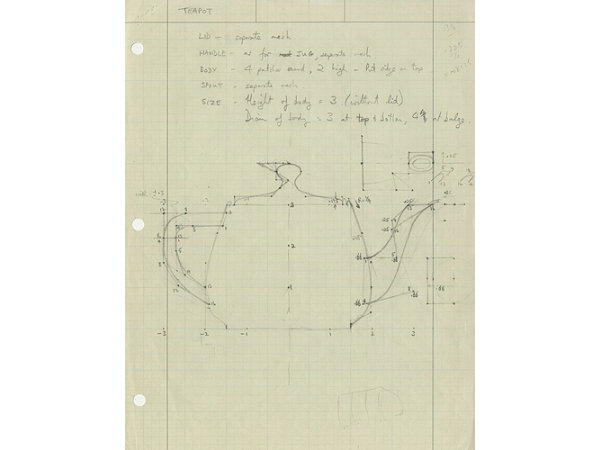
\includegraphics[scale=0.40]{utah_teapot_drawing.jpg}
\caption{Facsimile of the original 'Utah Teapot' drawing.}
\label{fig:utah_teapot_drawing}
\end{minipage}
\hspace{0.25cm}
\begin{minipage}[b]{0.45\linewidth}
\centering
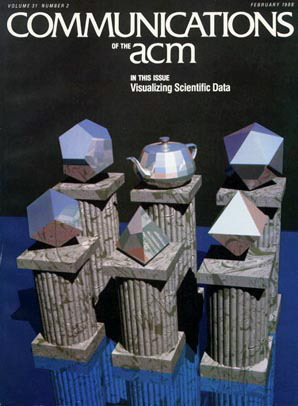
\includegraphics[scale=0.45]{utah_teapot_tribute.jpg}
\caption{The 'Teapotahedron' as the sixth platonic solid.}
\label{fig:utah_teapot_tribute}
\end{minipage}
\end{figure}\\
One famous tribute by Jim Arvo and Dave Kirk, from their '87 SIGGRAPH paper ``Fast Ray Tracing by Ray Classification'' shows six stone columns five of which are surmounted by the platonic solids (tetrahedron, cube, octahedron, dodecahedron, icosahedron) -- and the sixth has a teapot, see picture \ref{fig:utah_teapot_tribute}.

It is said that \textit{Newell} mentioned at a talk, that of all the things he has done for the world of Computer Graphics, the only thing he will be remembered for is: ``That damned teapot'' \citep[cf.][Copyright Computer History Museum]{Newell1975b}

\newpage
\vspace*{1ex}
\section{Proof -- Homeomorphism of regular quad meshes and tori}
\label{appendix4}

Meshes $\mathcal{M}_{reg}$ are regular if and only if all faces $\mathcal{F}_{i}$ have the same number of edges: $|E_{\mathcal{F}}|=const.$ and all vertices $\mathcal{V}$ have the same valence: $val(\mathcal{V}_{i})=const.$ -- this also means that every regular mesh must be manifold and thus satisfy the Euler-Poincaré characteristic, with $g$ being the genus of the mesh:
\begin{eqnarray}
\chi(\mathcal{M})=\mathcal{V}-E+\mathcal{F}=2(1-g)
\end{eqnarray}
A regular quad mesh $\mathcal{M}_{reg4}$ hence is a quadrilateral and each vertex is incident to exactly four edges, but since we count each edge twice, we get: $2\mathcal{V}=E$, accordingly each face has four edges, of which each edge is counted twice, so we have: $2\mathcal{F}=E$
\begin{eqnarray}
\mathcal{V}-E+\mathcal{F}=2(1-g)\\
\frac{E}{2}-E+\frac{E}{2}=2(1-g)\\
E-E=2(1-g)
\end{eqnarray}
Thus $\chi(\mathcal{M})=\mathcal{V}-E+\mathcal{F}=0$, which means $g=1$, i.e. a torus.
The argument for a regular triangle mesh is the same, with $3\mathcal{V}=E$ and $3\mathcal{F}=2E$ \citep[cf.][]{Shene2005}.
%Bild
\begin{figure}[ht]
\centering
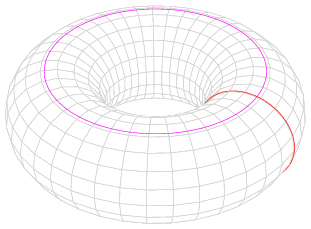
\includegraphics[width=0.50\textwidth]{torus_cycles.png}
\caption{Homology cycles on a torus (made with Mathematica, copyright wikipedia).}
\label{fig:torus_cycles}
\end{figure}

\newpage
\vspace*{1ex}
\section{Hausdorff distance}
\label{appendix5}

To be precise the Hausdorff distance is not a real distance, since any metric on a set must fulfill the requirement of symmetry, i.e. $d(x,y) = d(y,x)$ whereas $d_{\mathrm H}(x,y) \neq d_{\mathrm H}(y,x)$, so instead of a distance between $X$ and $Y$, the Hausdorff distance is more a distance from $X$ to $Y$ (sometimes also referred to as directed Hausdorff distance, but the terminology is not consistent).
For example in the case depicted in picture \ref{fig:hausdorff_asymmetry}, $d(\mathcal{S}, \mathcal{S}')$ of two open curves will remain much smaller than $d(\mathcal{S}', \mathcal{S})$, since here $d(A, \mathcal{S}) \ll d(B, \mathcal{S})$.
Thus a small one-sided distance does not necessarily imply a small overall distortion \citep[][cf. pp.705-706]{Aspert2002}.
This asymmetry is a property of \textit{maximin} functions, while \textit{minimin} functions are generally symmetric.
%Bild
\begin{figure}[ht]
\centering
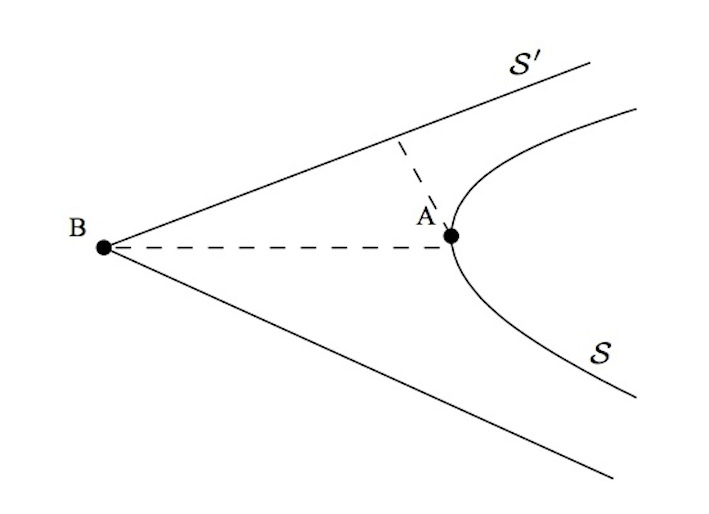
\includegraphics[width=0.33\textwidth]{hausdorff_asymmetry.jpg}
\caption{Asymmetry of the one-sided Hausdorff distance $d(\mathcal{S}, \mathcal{S}') \ll d(\mathcal{S}', \mathcal{S})$}
\label{fig:hausdorff_asymmetry}
\end{figure}\\
An important fact to reckon is that the Hausdorff distance is very sensitive to even one single outlying point $p_{d}$.
For example, consider $\mathcal{M}_{A} = \mathcal{M}_{B} \cup p_{d}$, where the point $p_{d}$ is at a large distance $d$ from any point of $\mathcal{M}_{A}$.
In this case $d_{\mathrm H}(\mathcal{M}_{A},\mathcal{M}_{B}) = d$, solely determined by the point $p_{d}$.\\
In our application scenario this is not of pivotal consideration, as every vertex of a decimated mesh has a 1-1 correspondent in the original mesh, but in general it is advisable to use a generalization of the Hausdorff distance.
It is given by taking the $k^{th}$ ranked distance rather than just the maximum:
\begin{equation} \label{eq:k_hausdorff}
d^{k}_{\mathrm H}(\mathcal{M}_{A},\mathcal{M}_{B}) = k^{th}\{\inf_{ p \in \mathcal{M} ~ p' \in \mathcal{M}'} d(p,p')\}
\end{equation}
For a good overview of the research that has been done in the recent years on the subject, as well as best practices for the implementation, see \citep[][]{Barton2010}.

\newpage
\vspace*{1ex}
\section{The house with two rooms}
\label{two_rooms}

A space having the homotopy type of a point is called contractible, this is trivially true for any unit ball $\mathcal{D}^{n}$ in $\mathbb{R}^{n}$.
Here is an example of a $2$-dimensional subspace of $\mathbb{R}^{3}$, known as ``The house with two rooms'' or ``Bing's house'', which is contractible but not in any obvious way.
%Bild
\begin{figure}[ht]
\centering
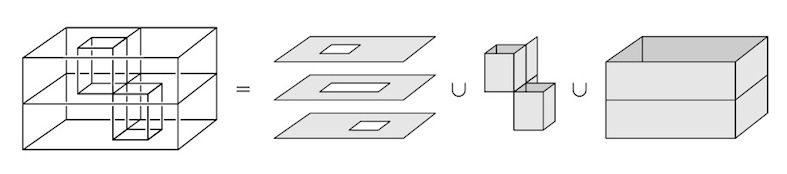
\includegraphics[width=1.00\textwidth]{two_rooms.jpg}
\caption{Decomposition of the retractable surface into its parts.}
\label{fig:two_rooms}
\end{figure}\\
To build this space, we have to start with a box divided into two chambers by a horizontal rectangle.
Access to the two chambers from outside the box is provided by two vertical tunnels.
The upper tunnel is made by punching out a square from the top of the box and another square directly below it from the middle horizontal rectangle, then inserting four vertical rectangles, the walls of the tunnel.
This tunnel allows entry to the lower chamber from outside the box.
The lower tunnel is formed in similar fashion.
Finally, two vertical rectangles are inserted to form ‘support walls’ for the two tunnels.
The resulting space is homeomorphic to the unit ball: $\mathrm{X} \simeq \mathcal{D}^{3} \simeq point$.
However, it is quite a challenging exercise to see exactly what this deformation retraction looks like.\\
To see this, imagine forming it from a ball of clay by pushing a finger into the ball to create the upper tunnel, then gradually hollowing out the lower chamber, and similarly pushing a finger in to create the lower tunnel and hollowing out the upper chamber.\\
The house has a visually obvious $2$-simplex structure. The $\sigma^{0}$ are the vertices where three or more of the depicted edges meet, and the $\sigma^{1}$ are the interiors of the edges connecting these vertices  and the $\sigma^{2}$ are the components of
the remainder of the space.
If counted, one finds there are 29 $\sigma^{0}$, 51 $\sigma^{1}$, and 23 $\sigma^{2}$, with the alternating sum $29-51+23 = 1$, the Euler characteristic \citep[][cf. pp.4-6]{Hatcher2002}.

\newpage
\vspace*{1ex}
\section{Proof -- Why P2 is not embeddable}
\label{appendix7}

The following proof was included, simply, for its intrinsic beauty.
The projective plane $\mathrm{P}^{2}$, sometimes called a twisted sphere, is the closed surface obtained by pasting a $2$-cell $\mathrm{e}^{2}$ and a Möbius band $\mathcal{M}$ together along their boundaries.\\
Recall that a trivial circle bounds a $2$-cell in $\mathbb{R}^{3}$ that is disjoint from all other curves, otherwise it is non-trivial.
Now, consider a set of six points in $\mathbb{R}^{3}$, and assume that each pair of these points is connected by a simple curve such that the curves meet only at their endpoints.
Such a figure is called a complete $6$-graph, denoted $\mathrm{K}6$, see figure \ref{fig:proof_embedded_1}:
%Bild
\begin{figure}[ht]
\centering
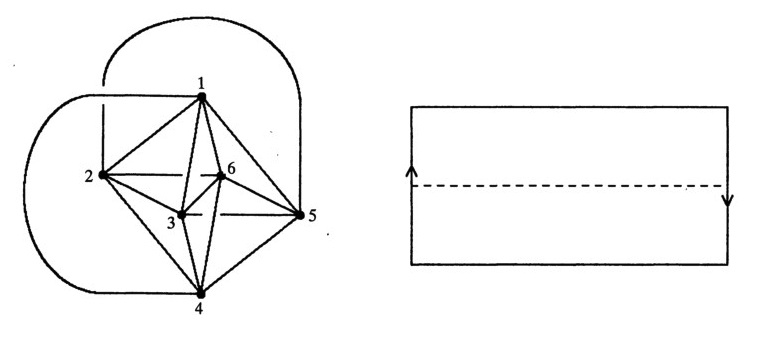
\includegraphics[width=0.80\textwidth]{proof_embedded_1.jpg}
\caption{Left: A complete $6$-graph; Right: Möbius band with dotted meridian.}
\label{fig:proof_embedded_1}
\end{figure}\\
To proof the theorem we need one corollary, the so called 'Link Appearing Theorem': \textit{Any complete $6$-graph in $\mathbb{R}^{3}$ contains a pair of disjoint cycles that form a non-triviallink} \citep[proven by:][]{Conway1983}.
In figure \ref{fig:proof_embedded_1} the pair of cycles $[1,3,5]$ and $[2,4,6]$ form such a non-trivial link\footnote{ Initially I found it hard to ``see'' these cycles, it helps to picture the two intertwined rings like two links of a chain.}.
Furthermore we define the meridian $\mathrm{C}$ of a Möbius band $\mathcal{M}$, as the line segment connecting the midpoints of the to-be-identified sides, see the dotted line in \ref{fig:proof_embedded_1}.
It represents a simple closed curve and for any embedding of $\mathcal{M}$ in $\mathbb{R}^{3}$, the pair $\{\partial \mathcal{M}, C\}$ form a non-trivial link\footnote{ A fun way to practically test this lemma, is to glue a paper strip so it forms a Möbius band and then cut it along the meridian. Thus getting an even more twisted band, cutting its meridian one more time, separates the two non-trivial links, which results in two independent but chained up bands of paper: $\beta^{0}=1\, \xrightarrow{double~meridian~cut}\, \beta^{0}=2$.}.\\
Consider the Möbius band represented in figure \ref{fig:proof_embedded_2}.
Each pair of the six points $\{1, 2, \dots,6\}$ is indeed, connected by a simple curve, making it a representation of $\mathrm{K}6$.
It contains ten pairs of disjoint cycles, each bounding a $2$-cell that is disjoint from the others.
For example, the cycle $[1,3,5]$ bounds the $2$-cell shaded in figure \ref{fig:proof_embedded_2}.
Hence, as nine pairs of cycles of $\mathrm{K}6$, other than $[1,3,4]$ and $[2,5,6]$ are trivial links, it follows with the 'Link Appearing Theorem' that these two must be non-trivial, i.e. the meridian and the boundary.
\begin{figure}[ht]
\centering
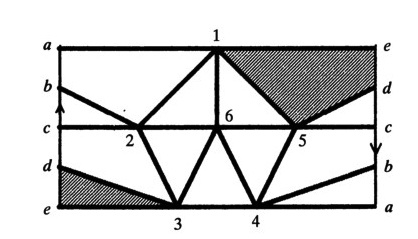
\includegraphics[width=0.60\textwidth]{proof_embedded_2.jpg}
\caption{A Möbius band built from a complete $6$-graph, $\mathrm{K}6$.}
\label{fig:proof_embedded_2}
\end{figure}\\
Now briefly suppose, that it was possible to embedded $\mathrm{P}^{2}$ in $\mathbb{R}^{3}$.
This would mean, that by removing an open $2$-cell from the surface we get, by definition, a Möbius band represented by $\mathcal{M}$.
Then, the boundary $\partial \mathcal{M}$ together with the meridian $\mathrm{C}$ form a non-trivial link, like two links of a chain.
But in consequence this would mean that $\mathrm{C}$ and the $2$-cell, as it is bound by $\partial \mathcal{M}$, must intersect each other at some point.
This is a contradiction, as the meridian is not intersected, as can be seen in the figure.
Therefore it is only possible to immerse $\mathrm{P}^{2}$ but impossible to embed it in $\mathbb{R}^{3}$, as it will always self intersect\footnote{ Basically the difference between an immersion and an embedding is that the immersion allows self-intersections. See figure \ref{fig:nonorientable_surfaces} for examples of a $\mathrm{P}^{2}$ immersion.}, see also the original publication \citep[][pp.862-864]{Maehara1993}.


\newpage
\vspace*{1ex}
\section{XYZ}
\label{appendix8}

Lorem ipsum.

\newpage
%\vspace*{1ex}
\section{Glossary -- Topology}
\label{appendix_glossary}

During my work on this thesis, I often found myself checking back with online resources to clarify certain expression.
This stems from the fact that on the one hand, topology is axiomatic in its nature and therefore relies on exact definitions rather than intuition, and on the other hand that there are deviant usages of nomenclature throughout the different fields that concern themselves with the topic.
Following is a short glossary that was a handy companion during the reading sessions.
I compiled it mainly from these resources: \href{http://mathworld.wolfram.com}{Wolfram MathWorld} -- which is an extensive pool of definitions, and some dedicated glossaries: \href{http://www.math.ucdavis.edu/profiles/glossary.html}{UC Davis -- Topology Index}, \href{http://www.ornl.gov/sci/ortep/topology/defs.txt}{Topology Atlas Glossary} and \href{http://en.wikipedia.org/wiki/Glossary_of_topology}{Wikipedia -- Glossary of topology}:
\vspace*{1ex}
\begin{description}
\begin{tiny}
\item[absolut retract] Let $\mathcal{K}$ be a class of topological spaces that is closed under homeomorphism, and let $\mathbb{X}_{1}, \mathbb{X}_{2} \in \mathcal{K}$. If $\mathbb{X}_{1} \subseteq \mathbb{X}_{2}$, is a retract for every element, i.e. there is a continuous map $f : \mathbb{X}_{2} \rightarrow \mathbb{X}_{1}$ such that for all elements in $\mathbb{X}_{1} : f(x) = x$, then $\mathbb{X}_{1}$ is a retract for the class $\mathcal{K}$. 
\item[algebraic geometry] Traditionally, the geometry of solutions in the complex numbers to polynomial equations. Modern algebraic geometry is also concerned with algebraic varieties, which are a generalization of such solution sets, as well as solutions in fields other than complex numbers, for example finite fields.
\item[algebraic topology] The branch of topology concerned with homology and other algebraic models of topological spaces.
\item[approach space] An approach space is a generalization of metric space based on point-to-set distances, instead of point-to-point.
\item[arc] Homeomorphic image of a closed line interval.
\item[automorphism] An isomorphism of a group with itself.
\item[basis] A basis for a topological space $\mathbb{X}$ is a collection of open sets that contain "arbitrarily small" neighborhoods of every point of $\mathbb{X}$. Specifically, for every point $x \in \mathbb{X}$, and for every open set $\mathbb{U}$ containing $x$, the collection must include a neighborhood of $x$ lying within $\mathbb{U}$. 
\item[boundary] The boundary (or frontier) of a set is the set's closure minus its interior. Equivalently, the boundary of a set is the intersection of its closure with the closure of its complement. The boundary of a set $\mathrm{A}$ is denoted by $\partial \mathrm{A}$ or $bd ~\mathrm{A}$. The boundary $\partial \mathbb{M}$ of a manifold is the set of points of it that have
boundary patches. The boundary of an $n$-manifold M is an (n-1)-manifold. A $n$-boundary must be a $n$-cycle.
\item[bounded] A set in a metric space is bounded if it has finite diameter. Equivalently, a set is bounded if it is contained in some open ball of finite radius. A function taking values in a metric space is bounded if its image is a bounded set.
\item[characteristic class] A kind of homological model for a decoration or property of a manifold or other topological space. The simplest characteristic class describes how a manifold fails to be orientable, that is, in which directions a being can travel in the manifold and reverse its handedness.
\item[circle packing] An arrangement of round disks in the euclidean-space{Euclidean} or hyperbolic plane or on the round sphere such that no two disks overlap with non-zero area. Depending on the context, the circles may or may not be the same size. A theorem of Koebe, revived by Thurston, states that given any planar graph, there is a circle packing with a circle for each vertex of the graph and kissing circles for each edge.
\item[classification] The goal in a branch of mathematics of providing an exhaustive list of some type of mathematical object with no repetitions. Example: The classification of 3-manifolds is one of the outstanding problems in topology. With the advent of computers, one weak but precise way to state a classification problem is to ask whether there is an algorithm to determine whether two given objects are equivalent.
\item[codimension] In general, if a mathematical object sits inside or is associated to another object of dimension $n$, then it is said to have codimension $k$ if it has dimension $n-k$.
\item[cohomology] Cohomology is an invariant of a topological space, formally dual to homology, and so it detects holes in a space. Cohomology has more algebraic structure than homology, making it into a graded ring (with multiplication given by the so-called 'cup product'), whereas homology is just a graded Abelian group invariant of a space. 
\item[combinatorial geometry] The visual study of discrete and finite structures, and the study of discrete and finite possibilities for the arrangement or features of geometric objects.
\item[compact] A topological space is compact if every collection of open sets that covers the space has a finite subset that also covers the space. The compact subspaces of $\mathbb{R}^{n}$ are the closed and bounded sets.
\item[complex manifold] A manifold with complex coordinates; its ordinary or real dimension is then twice its complex dimension.
\item[completely regular] A space is completely regular if, whenever C is a closed set and x is a point not in C, then C and {x} are functionally separated.
\item[conformal] Angle-preserving or angle-defining. The Mercator map is a conformal map of the Earth because angles are true. A conformal structure on a manifold defines angles between curves segments on the manifold but not their lengths.
\item[connected sum] 1. A manifold formed from two others by removing balls and gluing along the resulting spherical boundary.
2. The analogous operation for knots; a band-connected sum in which the band connects the knots in the simplest possible way (by piercing the separating sphere only once)..
\item[contractible] A space $\mathbb{X}$ is contractible if the identity map on $\mathbb{X}$ is homotopic to a constant map, i.e. a space is contractible if it can be shrunk to a point within itself. The homotopy that does this is called a 'contraction'. Every contractible space is simply connected.
\item[convolution] A convolution of two planar regions is the set of all vector sums of a point in one region with a point in the other.
\item[curvature] In Riemannian geometry, usually means the intrinsic curvature of a manifold with a Riemannian metric.  The curvature at a point is positive (negative) if the sum of the angles of a small approximate triangle at that point is greater than (less than) $180^{\circ}$ degrees.
\item[cyclically symmetric, self-complementary plane partition] A plane partition in a cube which is symmetric under sending the x axis to the y axis, y to z, and z to x, and at the same time is equal to its complement; the set of cubes in the box not in the plane partition considered again as a plane partition by inverting all three axes. Equivalently, a lozenge tiling of a regular hexagon invariant under 60 degree rotation.
\item[deformation retract] A subspace $\mathrm{A} \subset \mathbb{X}$ is a deformation retract if $\mathbb{X}$ can be shrunk
down to $\mathrm{A}$ without moving any point of $\mathrm{A}$. The homotopy that does the shrinking is called a 'deformation retraction'.
\item[degenerate diffusion] A diffusion process that only allows diffusion in prespecified directions instead of in every direction.
\item[diffeomorphism] A bijection between two manifolds that preserves all smooth structure.
\item[differential geometry] The general study of smooth manifolds decorated by continuous structures such as foliations, Riemannian metrics, and symplectic structures. Riemannian geometry is a disproportionate part of differential geometry.
\item[discrete space] A space X is discrete if every subset of X is open. We say that X carries the discrete topology.
\item[embedding] A mapping into a space whose image is homeomorphic to the domain. The parametrization of a submanifold by means of a standard model. A knotted sphere in $4$-space is an embedding of the familiar round sphere.
\item[foliation] A decoration of a manifold in which the manifold is partitioned into sheets of some lower dimension, and the sheets are locally parallel. (More technically, the foliated manifold is locally homeomorphic to a vector space decorated by cosets of a subspace).
\item[functor] A correspondence from one category to another mapping objects to objects and preserving morphisms.
\item[fundamental group] A group, often non-abelian, that rather fully describes the periodicity or the 1-dimensional holes in a topological space.
\item[geodesic] On a Riemannian manifold or some other metric space, a curve which is the shortest path between any two points on it that are sufficiently close together.
\item[geometric function theory] The study of the geometry in the complex plane of complex analytic functions, in particular the relation between the image of the unit disk of an analytic function and its power series.
\item[Geometrization Conjecture] The conjecture of Thurston that, after cutting along essential spheres and tori, every compact 3-manifold admits a special Riemannian metric known as a geometry, usually hyperbolic geometry. The conjecture subsumes the Poincaré conjecture and many other standard conjectures about 3-manifolds, and constitutes a classification of 3-manifolds.
\item[Gromov norm] An invariant associated with the homology of a topological space that measures how many simplices are needed to represent a given homology class.
\item[group] A mathematical system consisting of elements from a set and a binary operation such that they obey: Associativity and closure for the elements, as well as having an identity element and an inverse element.
\item[homeomorphism] A bijection between two topological spaces that preserves all continuous structure; the basic notion of equivalence in topology. If $\mathbb{X}_{1}$ and $\mathbb{X}_{2}$ are spaces, a homeomorphism from $\mathbb{X}_{1}$ to $\mathbb{X}_{2}$ is a bijective function $f : \mathbb{X}_{1} \rightarrow \mathbb{X}_{2}$ such that $f$ and $f^{-1}$ are continuous. The spaces $\mathbb{X}_{1}$ and $\mathbb{X}_{2}$ are then said to be homeomorphic. From the standpoint of topology, homeomorphic spaces are identical.
\item[] A space $\mathbb{X}$ is homogeneous if, for every x and y in $\mathbb{X}_{1}$, there is a homeomorphism $f : \mathbb{X}  \rightarrow \mathbb{X}$ such that $f(x) = y$. Intuitively, the space looks the same at every point. Every topological group is homogeneous.
\item[homological algebra] The algebraic study of the homology and cohomology of manifolds and other mathematical objects. Homological algebra is a grand generalization of linear algebra.
\item[homology/singular homology] Homology is an algebraic object associated to a manifold or another mathematical object which gives a measure of the number of holes in the object -- manifolds form a homology when they form the boundary of a higher-dimensional manifold inside the manifold in question. The homology of a topological space has a relatively technical definition, but it is relatively easy to compute and study with tools from linear algebra.
\item[homotopy/homotopic maps] Two continuous maps f, g : $\mathbb{X}_{1} \rightarrow \mathbb{X}_{2}$ are homotopic (in $\mathbb{X}_{2}$) if there is a continuous map $H : \mathbb{X}_{1} \times [0, 1] \rightarrow \mathbb{X}_{2}$ such that $H(x, 0) = f(x)$ and $H(x, 1) = g(x)$ for all x in $\mathbb{X}_{1}$. Here, $\mathbb{X}_{1} \times [0, 1]$ is given the product topology. The function $H$ is called a homotopy (in $\mathbb{X}_{2}$) between $f$ and $g$.
\item[hyperbolic geometry] In modern terms, hyperbolic geometry is the study of manifolds with Riemannian metrics with constant negative curvature. The hyperbolic plane is a particular hyperbolic manifold which is in a sense universal among hyperbolic surfaces; similarly there is also hyperbolic n-space. Escher's circle limit prints are excellent illustrations of the hyperbolic plane.
\item[immersion] A locally but not globally smoothly invertible mapping of one manifold into another. The image may have self-intersections. For example, the figure-8 is an immersion of the circle in 2D.
\item[invariant] In topology, a number, polynomial, or other quantity associated to a topological object such as a knot or 3-manifold which depends only on the underlying object and not on its specific description or presentation.
A topological invariant is a property which is preserved under homeomorphism. For example, compactness and connectedness are topological properties, whereas boundedness and completeness are not. Algebraic topology is the study of topologically invariant abstract algebra constructions on topological spaces.
\item[interior] The interior of a set is the largest open set contained in the original set. It is equal to the union of all open sets contained in it. An element of the interior of a set $\mathrm{A}$ is an interior point of $\mathrm{A}$.
\item[isometric isomorphism] If $\mathbb{M}_{1}$ and $\mathbb{M}_{2}$ are metric spaces, an isometric -- a mapping which preserves the metric -- isomorphism from $\mathbb{M}_{1}$ to $\mathbb{M}_{2}$ is a bijective isometry $f : \mathbb{M}_{1} \rightarrow \mathbb{M}_{1}$. The metric spaces are then said to be isometrically isomorphic. From the standpoint of metric space theory, isometrically isomorphic spaces are identical.
\item[Jacobian variety] A space associated to a Riemann surface defined most succinctly as the complex cohomology (as a vector space) divided by the integral cohomology (as a lattice). It is simultaneously a complex manifold, an algebraic variety, and a Lie group.
\item[Jones polynomial] A famous invariant of knots and links discovered by Vaughan Jones. It has several extremely elementary definitions and at the same time involves deep mathematics.
\item[kernel] In algebra, the set of vectors annihilated (sent to zero) by a matrix, linear operator, homomorphism, or any similar function. In analysis, a continuous analogue of a matrix. Given a vector space of functions of a parameter or functions on a manifold, an operator may have a kernel or matrix whose rows and columns are indexed by the parameter or by points on the manifold.
\item[knot/link] A link is a collection of disjoint circles lying in a 3-manifold, often but not always Euclidean 3-space or the 3-sphere. A knot is link which happens to be a single circle. Manifold topologists usually study tame knots and links, which can be represented by smooth or polygonal curves, but there are also wild links which are infinitely knotted. Ordinary knots and links were topologically classified (in a certain sense) by Haken and Thurston.
\item[lamination] A decoration of a manifold in which some subset is partitioned into sheets of some lower dimension, and the sheets are locally parallel. It may or may not be possible to fill the gaps in a lamination to make a foliation.
\item[lattice] A periodic arrangement of points such as the vertices of a tiling of space by cubes or the positions of atoms in a crystal. More technically, a discrete abelian subgroup of an n-dimensional vector space which not contained in an n-1-dimensional vector space. Lattices play a central role in the theory of Lie groups, in number theory, in error-correcting codes, and many other areas of mathematics.
\item[Lie algebra] An algebraic structure on a vector space which describes multiplication of elements of a Lie group which are very close to the identity (infinitesimal transformations). Lie algebras are almost as important as their comrades-at-arms, Lie groups.
\item[Lie group] A group (in the sense of abstract algebra) which is at the same time a manifold. Example: The group of rotations in n dimensions is a Lie group of dimension n(n-1)/2. Lie groups are fundamental objects in mathematics and physics, especially quantum field theory.
\item[loop space] Given a topological space $\mathbb{X}$, its loop space is the topological space of all continuous functions from a circle to $\mathbb{X}$. Loop spaces are important examples of new topological spaces formed from old ones, as well as examples of infinite-dimensional spaces in mathematics.
\item[loop and sphere theorems] Two foundational theorems in 3-manifold topology, proved by Papakyriakopoulos in the 1950's. The loop and sphere theorems generalize Dehn's lemma, which asserts that if a knot in three dimensions bounds a disk which intersects itself in its interior, the disk can be simplified to remove all self-intersection and the knot must be trivial.
\item[loop, trivial] The trivial loop is the loop that takes every point to its basepoint. Formally, if $\mathbb{X}$ is a topological space and $x \in \mathbb{X}$, the trivial loop based at $x$ is the map $f : [0,1] \rightarrow \mathbb{X}$ given by $f=x$ for all arguments -- therefore (trivially) fulfilling the requirement of a loop: A map of the unit interval [0,1] into a space with the same beginning and end points, i.e. $f(0)=f(1)$.
\item[metrizable] For a topological space, the property that there exists a metric compatible with the topology. To say that a topological space is metrizable is to treat it as a metric space, but without distinguishing any specific or preferred distance function.
\item[Moore space] A Moore space is a developable regular Hausdorff space.
\item[neighbourhood] A neighbourhood of a point x is a set containing an open set which in turn contains the point x. More generally, a neighbourhood of a set S is a set containing an open set which in turn contains the set S. A neighbourhood of a point x is thus a neighbourhood of the singleton set \{x\}. (Note that under this definition, the neighbourhood itself need not be open. Many authors require that neighbourhoods be open; be careful to note conventions.)
\item[non-abelian] Non-commutative or order-dependent. For example, the group of manipulations of the Rubik's cube is non-commutative because the state of the cube depends greatly on the order that moves are performed on it.
\item[orbifold] A topological object defined by Thurston which is locally modelled by Euclidean spaces divided by finite groups of symmetries. Orbifolds are manifolds with singularities such as reflection surfaces, where they resemble manifolds with boundary, and cone lines, where they are modelled (in the direction perpendicular to the cone line) by a cone with an angle of 360/n degrees for some n.
\item[partition of unity] A partition of unity of a space $\mathbb{X}$ is a set of continuous functions from $\mathbb{X}$ to $[0, 1]$ such that any point has a neighbourhood where all but a finite number of the functions are identically zero, and the sum of all the functions on the entire space is identically $1$.
\item[path-connected component] A path-connected component of a space is a maximal nonempty path-connected subspace. The set of path-connected components of a space is a partition of that space, which is finer than the partition into connected components. The set of path-connected components of a space $\mathbb{X}$ is denoted $\pi_{0}(\mathbb{X})$.
\item[path homozopy] A homotopy between paths that fixes their endpoints; or the relation of being path-homotopic. Two paths are path-homotopic if there is a path homotopy between them.
\item[PL flow] A motion on a space or a manifold, akin to a flow given by a vector field, in which every particle in a given simplex of some triangulation moves with constant velocity and in the same direction, so that the particle trajectories are polygons.
\item[pleated surface] A surface in Euclidean or hyperbolic space which resembles a polyhedron in the sense that it has flat faces that meet along edges. Unlike a polyhedron, a pleated surface has no corners, but it may have infinitely many edges that form a lamination.
\item[Poincaré conjecture] The conjecture that a closed, simply-connected 3-manifold must be homeomorphic to the 3-sphere. Many mathematicians, including Poincaré himself, have presented incomplete and incorrect proofs of the conjecture. It was finally proven by \textit{Grigori Perelman} who was awarded the Field Medal for it, but declined it. It is the only solved Millennium problem.
\item[polyhedron] A region in Euclidean space which consists of flat facets with flat edges. More technically, a polyhedron must locally be a cone over a lower-dimensional polyhedron. It is sometimes but not always implicitly assumed that a polyhedron is a manifold, a topological sphere or ball, or a convex set.
\item[polytope] The n-dimensional generalization of a polygon or a polyhedron.
\item[projective plane] A 2-manifold obtained by gluing a Möbius strip and a disk along their circle boundaries.
\item[quasicompact] Some authors define "compact" to include the Hausdorff separation axiom, and they use the term quasicompact to mean what we call in this glossary simply "compact" (without the Hausdorff axiom). This convention is most commonly found in French, and branches of mathematics heavily influenced by the French.
\item[quotient map] If $\mathbb{X}_{1}$ and $\mathbb{X}_{2}$ are spaces, and if f is a surjection from $\mathbb{X}_{1}$ to $\mathbb{X}_{2}$, then $f$ is a quotient map (or identification map) if, for every subset $U$ of $\mathbb{X}_{2}$, $U$ is open in $\mathbb{X}_{2}$ if and only if $f^{-1}(U)$ is open in $\mathbb{X}_{1}$. In other words, $\mathbb{X}_{2}$ has the f-strong topology. Equivalently, $f$ is a quotient map if and only if it is the transfinite composition of maps $\mathbb{X}_{1} \rightarrow \mathbb{X}_{1}/\mathbb{X}_{3}$, where $\mathbb{X}_{3} \subset \mathbb{X}_{1}$ is a subset. Note that this doesn't imply that f is an open function.
\item[quotient space] If $\mathbb{X}_{1}$ is a space, $\mathbb{X}_{2}$ is a set, and $f : \mathbb{X}_{1} \rightarrow \mathbb{X}_{2}$ is any surjective function, then the quotient topology on $\mathbb{X}_{2}$ induced by f is the finest topology for which f is continuous. The space $\mathbb{X}_{1}$ is a quotient space or identification space. By definition, $f$ is a quotient map. The most common example of this is to consider an equivalence relation on $\mathbb{X}_{1}$, with $\mathbb{X}_{2}$ the set of equivalence classes and f the natural projection map. This construction is dual to the construction of the subspace topology.
\item[random triangulation] A triangulation of a surface or other manifold chosen by a random process. In a particularly interesting case, one considers all triangulations with a fixed, large number of triangles to be equally likely.
\item[representation/linear representation] A realization of a group, Lie group, or Lie algebra by matrices or linear transformations. More technically, a homomorphism from a group to a group of matrices.
\item[representation theory] The study of linear representations of groups, Lie groups and Lie algebras.
\item[resolvable] A topological space is called resolvable if it is expressible as the union of two disjoint dense subsets.
\item[Reuleaux polytope] A convex body in the plane or in higher dimensions which, like a Reuleaux triangle, consists of pieces of round spheres, each centered at one of the corners of the convex body.
\item[Riemann sphere] A topological sphere consisting of the complex plane and the point at infinity; an example of a Riemann surface.
\item[Riemannian geometry] The study of curvature and other properties of Riemannian metrics on manifolds. Sometimes also called differential geometry.
\item[round] In topology, the terms circle and sphere refer to topological objects and not geometric ones, so that the surface of an egg shape is also considered a sphere.  A round sphere, then, is a sphere with constant curvature, i.e. a sphere in the normal sense of geometry.
\item[simplex] The n-dimensional generalization of the triangle and the tetrahedron; a polytope in n dimensions with n+1 vertices.
\item[simplicial] Made up of simplices. For example, a simplicial polytope has simplices as faces and a simplicial complex is a collection of simplices pasted together in any reasonable vertex-to-vertex and edge-to-edge arrangement.
\item[smooth] Generally meaning, possessing infinitely many derivatives. For example, $\sin(x)$ is a smooth function, while $|x|^{3}$ is not.  Manifolds are smooth if they can be defined or described by smooth functions, which implies the possession of continuous tangents.
\item[spectral sequence] Is a means of computing homology groups by taking successive approximations. Spectral sequences are a generalization of exact sequences, and since their introduction in the 1940s by \textit{Jean Leray}, they have become an important research tool, particularly in homotopy theory. Roughly speaking, a spectral sequence is a system for keeping track of collections of exact sequences that have maps between them, thus describing intricate relationships among homology and cohomology groups coming from geometric situations such as fibrations and from algebraic situations involving derived functors.
\item[stratifiable] A topological space is stratifiable if it can be decomposed into shells which are similar to the shells that are a fixed distance from a point in a metric space.
\item[SU(2)] The 3-dimensional Lie group of 2 x 2 unitary matrices; the most common Lie group in mathematics and physics after the circle.
\item[topological complexity] A lower bound on computational complexity introduced by Smale that involves topology. A task with high computational complexity requires a computer to make many decisions, sometimes arbitrary decisions, to untangle the topology of the space of possible inputs or outputs or the space of possibilities for an intermediate quantity.
\item[topological space] The basic object of topology; a formal model of the qualitative way in which something is connected to itself. The technical definition is that a topological space is a set X together with distinguished subsets called open sets or open neighborhoods, such that the the empty set and X are open, the intersection of two open sets is open, and the union of an arbitrary collection of open sets is open. See also the definition of space.
\item[train track] A graph drawn on a surface such that every vertex has degree three, and such that all three edges meeting at a vertex have a common tangent, two edges on one side and one on the other. Every lamination of a surface is approximately parallel to, or carried by, a train track.
\item[weak topology] The weak topology on a set, with respect to a collection of functions from that set into topological spaces, is the coarsest topology on the set which makes all the functions continuous.
\item[weight] The weight of a space $\mathbb{X}$ is the smallest cardinal number $\mathrm{K}$ such that $\mathbb{X}$ has a base of cardinal $\mathrm{K}$. (Note that such a cardinal number exists, because the entire topology forms a base, and because the class of cardinal numbers is well-ordered.)

\end{tiny} 
\end{description}
